%TODO: What other methods exist? What are the differences? What are the difficulties with other methods? How does it compare to a baseline method?

%\href{https://www.math.leidenuniv.nl/scripties/BSC-Obbens.pdf}{Interisting stuff} \cite{obbens2014inference}

\subsection{Bayesian networks} \label{sec:bayes}
% 2 page

As the Markov network, the Bayesian network is also a method for representing probabilistic models with a graph. Since the roots of Bayesian networks lie in path analysis by Right in 1921 \cite{wright1921correlation} and 1934 \cite{wright1934method}, this method of representation is slightly older than the Markov networks, which was firstly introduced by Barlett in 1935 \cite{bartlett1935contingency}.

The main difference between the Bayesian and the Markov network is that the first one has directed edges whereas the second has undirected ones. Furthermore the Bayesian network is restricted to be acyclic. This means that the dependency between two random variables can never be mutual but only one-directional. Thus, the edge $(A, B)$ would indicate that $B$ depends on $A$ and that their is no path from $B$ to $A$, which means that $A$ is the cause and $B$ the effect in this particular relation.

In the contrary to Markov networks the Bayesian network is able to assign the parameters by using probabilities. Because of the condition, that the graph is an acyclic directed graph, the number of variables, on which a variable $X$ depends, is equal to the number of its incoming edges. Using conditional probability distributions (CPD) a probability is assigned to each assignment times the number of values of $X$. The sum of probabilities of a \textit{CPD} is equal to one. When inferring on a Bayesian network the factor multiplication is similar to the Markov network: Multiply the probabilities of \textit{CPDs}, such that the assignments match up. Figure \ref{fig:bayes} shows a simple Bayesian network with four binary variables and their conditional probability distributions. As described above the summation over the product of \textit{CPDs} is calculated for inferring on the Bayesian network. Equation shows an example calculation for computing $P(D = d_T).$ The result of the example inference is, that $D$ is with a certainty of 64\% true.

\begin{equation}
P(D = d_T)=\sum_A{\sum_B{\sum_C{P(A)P(B|A)P(C)P(d_T|B,C)}}} = 0.64
\label{eq:bayes}
\end{equation}

\begin{figure}[htpb]
  \centering
  	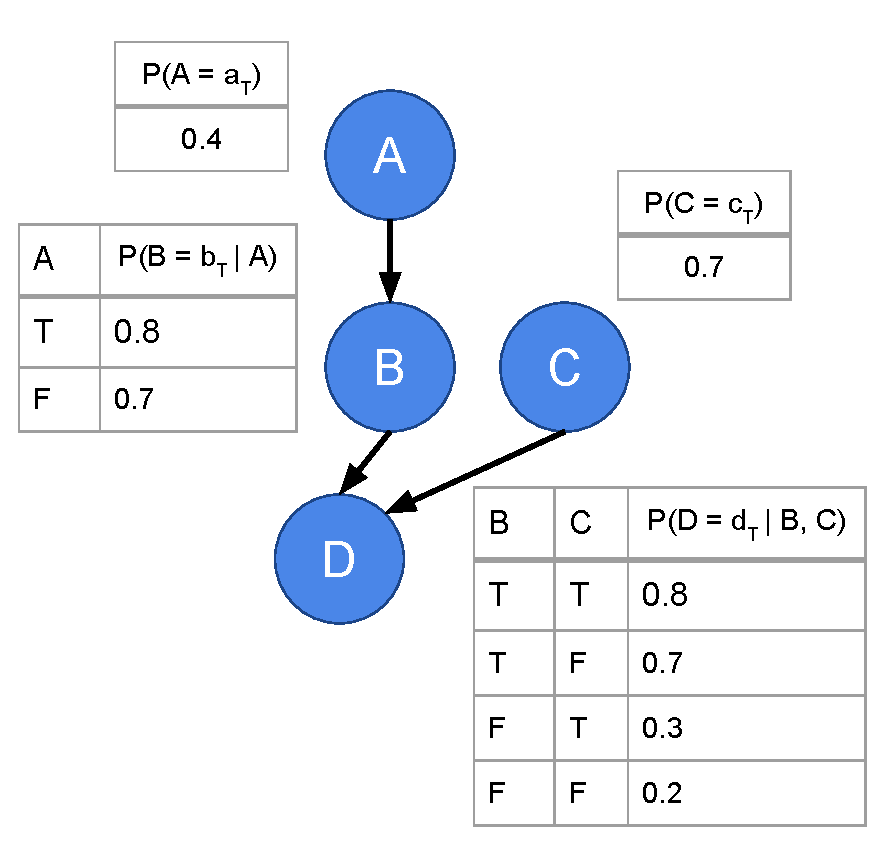
\includegraphics[scale=0.6]{img/bayes.pdf} 
  \caption{Examples of a Bayesian network including the conditional probability distributions}
  \label{fig:bayes}
\end{figure}

Since the affinities among assignments of random variables are expressed as probabilities, the adjustment of the parameters are not as flexible as in Markov networks.
% TODO: example, why is that?

In section \ref{sec:indep} the independences of a variable given a certain set of other variables was described as local Markov property using the Markov blanket for the Markov network. Also in Bayesian networks every node has a Markov blanket, for which holds that: Given the Markov blanket of a node, this node is independent from all variables unequal to the Markov blanket and the node itself. In Bayesian networks the Markov blanket includes the parents, the children and the other parents of the children. Using this property, the inference on those networks can be elevated dramatically in terms of computation time and space.

% TODO: example bayesian networks with cpd annotations

% TODO: Transformation of Bayesian network to Markov network and vise versa

%\subsection{Partially directed models}
% 1 page
% not sure of this
%- chapter 4.6


\subsection{Markov logic network} \label{sec:mln}
% 1.5 page

In 2006 Matthew Richardson and Pedro Domingos from the University of Washington in Seatle proposed to combine first-order logic with probabilistic graphical models and named it Markov logic network \cite{richardson2006markov}. This section firstly describes what a Markov logic network is and how it extends the Markov network and secondly discusses the benefits of this approach and what types of problems it confronts.

- first-order knowledge base set of sentences or formulas in first-order logic
- constants (objects), variables (range over the objects of the domain), functions (maps tuple of objects onto objects), predicates (relations between or attributes of objects)
- example of those
- terms and sentences

- assign weights to the sentences of the KB
- MLN is a set of pairs of first-order logic formulas and weights expressed in real numbers. the Markov network is defined by L and the finite set of constants of the domain 
 - a binary node for each predicate appearing in L
 - a binary feature for each formula, the weight of the feature is the weight of the formula
- example shown in \cite{richardson2006markov} with Anna and Bob smoking, cancer and Friends
% TODO: include figures

- inference
 - arbitrary queries of the form how likely does a formula $F_1$ holds given that $F_2$ holds? both in first-order logic and a finite set of constants, including all constants that appear in F1 and F2 \cite{richardson2006markov} and L is a MLN
  - use conditional probability and sum up all worlds where both are true divided by where F2 is true
  
- learning
 - learning the weights of the formulas
 - areas of application: classification, link prediction, social network modeling, object identification
 - Example for an learning application: Classifying Topics and Detecting Topic Shifts in Political Manifestos with a Markov logic network \cite{zirn2016classifying}


